\chapter{Simulator Use Cases}
\label{cap:uses}

This chapter presents the utilization of the InterSCSimulator to support other research during the last two years. Section \ref{sec:test} presents the utilization of the simulator to perform experiments on InterSCity Platform, a Smart City software platform. Section \ref{sec:paraisopolis} describes the simulation of different mobility scenarios in the Paraísopolis community in S\~ao Paulo. Section \ref{sec:vanet} presents the simulation of Vehicular Ah-Doc Networks (VANETs) aided by mobility traces generated from InterSCSimulator. Finally, Section \ref{sec:mobiity_model}

\section{InterSCity Platform Integration}

To test Smart City services and applications, we integrated the InterSCSimulator and InterSCity Platform. The InterSCity platform is an open source micro-services-based platform to enable collaborative research, development, and experiments in smart cities. The platform handles the mandatory requirements to support integrated smart city services and applications in different domains such as transportation, health-care, and environmental monitoring. The integration is performed in two ways:

\begin{itemize}

\item \textbf{Application Request: } The platform simulates the access of a person to a Smart City application deployed in the platform. To simulate it, the simulator makes an HTTP request to a platform service that sends a response with the data requested. The simulator must handle the response and change the behavior of the actor that sends the request.

\item \textbf{City Infrastructure: } The simulator is also capable of simulating city sensors which generate data and send to the platform. This data is sent to the platform using a queue system deployed in the platform.

\end{itemize}

Figure \ref{fig:integration} presents the integration of the platform and the simulator. The application request integration is at the top of the figure, showing that the simulator makes a request and receive a response from the platform. The City Infrastructure integration is at the bottom of the figure, showing that the simulator sends sensor data to the platform.

\begin{figure}[!htb]
\centering
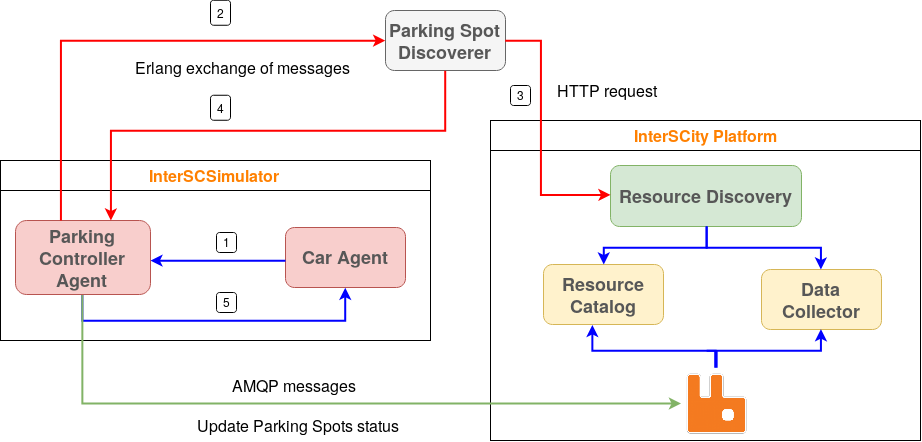
\includegraphics[width=0.8\textwidth]{figuras/chap-uses/integration.png}
\caption{Platform Response Time}
\label{fig:integration}
\end{figure}

The InterSCity research group tested a Smart Parking application using the simulator-platform integration. The scenario was: (1) a driver makes an HTTP request to the platform seeking a parking spot; (2) the platform sends a parking spot and its location; (3) the driver changes its route to go to the parking spot; (4) when the driver stops the car in the parking spots, update the state of the spot sensor in the platform. Steps 1, 2, and 3 are implemented using the application request integration, and step 4 using the city infrastructure integration.

\subsection{InterSCity Platform Scalability Experiments}
\label{sec:test}

The focus of InterSCity platform is to handle the required scalability of a Smart City platform. It is necessary because a Smart City will have thousands of applications and millions of users. The platform has to deal with a considerable variation in the load during the day. For example, a traffic application will be hugely used during the peak hour and normal use in the other hours.

As perform scalability experiments in real environments is not easy, the developers of the platform used the simulator integration to generate a massive workload to the platform. The simulated scenario was the Smart Parking application in the morning peak hour in the city of S\~ao Paulo. The simulation had more than 400 thousand simulated cars, and each car made one or more requests to the platform searching for a parking spot.

Figure \ref{fig:workload_interscity} presents the workload generated in the simulator. The number of requests increase with the passage of time and allow the verification of the behavior of the platform with the variation of the load. The figure presents the workload mean of 15 executions of the platform experiments.

\begin{figure}[!htb]
\centering
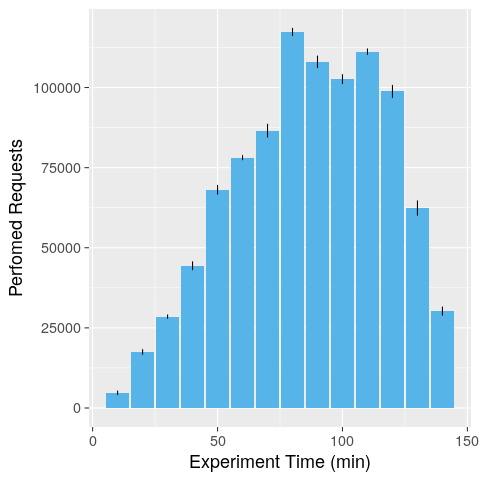
\includegraphics[width=0.6\textwidth]{figuras/chap-uses/load_mean.png}
\caption{Workload generated in the simulation}
\label{fig:workload_interscity}
\end{figure}

The simulator developers executed more than 50 experiments using the simulator, aiding them to find many problems in the platform implementation and achieve the desired scalability. Figure \ref{fig:response_time_interscity} presents the response time of the platform using the load of Figure \ref{fig:workload_interscity}. 

\begin{figure}[!htb]
\centering
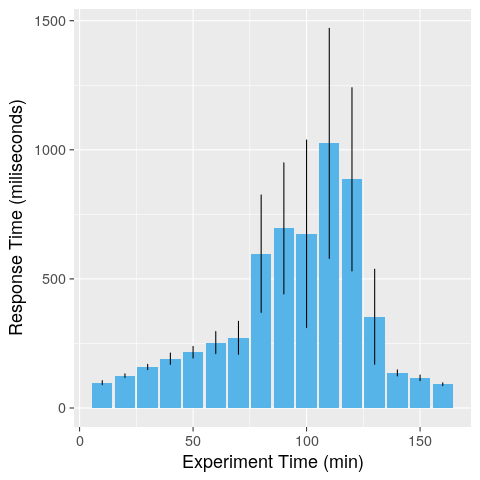
\includegraphics[width=0.6\textwidth]{figuras/chap-uses/response_time_mean.png}
\caption{Platform Response Time}
\label{fig:response_time_interscity}
\end{figure}



\section{Scenarios in Paraisópolis}
\label{sec:paraisopolis}

InterSCSimulator is useful to compare large-scale mobility scenarios. The Traffic Engineering Group from the Polytechnic School from the University of S\~ao Paulo used the simulator to study the impact of a subway line under construction in the city of S\~ao Paulo, especially in the Paraisópilis community, one of the largest poor neighborhoods of the city. This subway line will have two stations in the community, and it will have a significant impact on the population access to quality transportation.

In their work, they examined four simulated scenarios based on a city origin-destination survey and compared their travel time, financial cost, and carbon footprint of the simulated population. They based all the scenarios on realistic changes that might occur with the new subway line. Besides the OD, they also used data from the city buses and metro lines. They simulated the entire community population (approximately 44 thousand people) and other cars from the city to generate car traffic.

The simulation showed that the users of buses could benefit from a decrease in their travel time, and car uses can have economic benefits with the new subway line. For example, of the population that used cars in the original scenario, approximately 1,500 had their travel times decreased, and 4,000 had their travel times increased. The people that had their travel time increased by more than 30 minutes (around 2,000 people) are unlikely to change their travel mode. However, since the cost reduction can be very substantial (mainly when taking into consideration parking fees), even some of them might prefer the subway.

\begin{figure}[!htb]
\centering
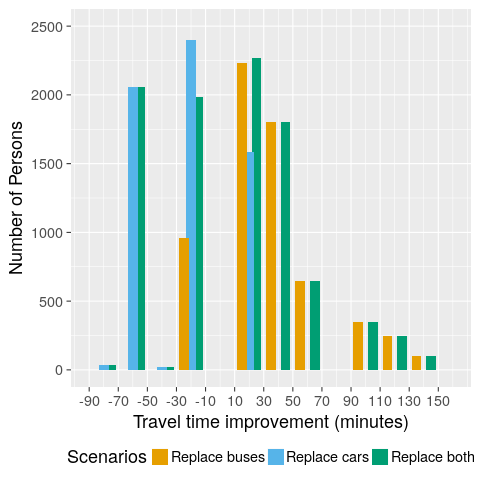
\includegraphics[width=0.6\textwidth]{figuras/chap-uses/hist_travel_time.png}
\caption{Travel time improvement}
\label{fig:travel_time}
\end{figure}

\section{VANETs Simulation}
\label{sec:vanet}

Using the S\~ao Paulo simulation presented in Chapter \ref{cap:sao_paulo} we generated mobility trace to enable tests and experiments of Vehicular Ah-Doc Networks (VANETs). The trace contains the events of all the cars of the simulation during an entire day. The advantage of this trace comparing with other traces available in the literature is the enormous amount of vehicles. While the trace generated in this research contains more than 4 million travels of buses and cars, the other traces contains less than 700 thousand travels.

To show the use of this trace, we converted the output of InterSCSimulator to the input format of NS-3\footnote{NS-3 -- https://www.nsnam.org/}, a popular network simulator. Listing \ref{list:trace_ns3} presents an example of a NS-3 input file.

\renewcommand{\thelstlisting}{\arabic{lstlisting}}
\begin{lstlisting}[caption=NS-3 input file, label=list:trace_ns3, upquote=true]
$node_(0) set X_-23.55084
$node_(0) set Y_-46.62869
$node_(0) set Z_ 0
$ns_ at 15451 "$node_(0) setdest -23.55084 -46.62869 0"
$node_(1) set X_-23.55084
$node_(1) set Y_-46.62869
$node_(1) set Z_ 0
$ns_ at 15469 "$node_(1) setdest -23.55084 -46.62869 0"
\end{lstlisting}

In the file, the lines starting with a \textdollar node, define the creation of network node in the NS-3. The lines starting with \textdollar ns represent the movements of the vehicles and occurs many times until the vehicle arrives at its destination. We used this file in an NS-3 simulation which creates a vehicular network based on the distance of the vehicles. The simulation generates a MAC address to each vehicle, and at each simulation steps it connects or disconnects the vehicles. Listing \ref{list:ns3_output} presents an example of the output of an NS-3 simulation.

\renewcommand{\thelstlisting}{\arabic{lstlisting}}
\begin{lstlisting}[caption=NS-3 Output, label=list:ns3_output, upquote=true]
15469 0 -23.5508 -46.6287 00:00:00:00:00:01 0 
15469 1 -23.5508 -46.6287 00:00:00:00:00:02 0 
15470 0 -23.5508 -46.6287 00:00:00:00:00:01 1 
00:00:00:00:00:02 
15484 2 -23.5508 -46.6287 00:00:00:00:00:03 0 
15485 0 -23.5517 -46.6279 00:00:00:00:00:01 2 
00:00:00:00:00:02 00:00:00:00:00:03 
\end{lstlisting}

Each line in the file corresponds to a vehicle in an instant of the simulation. The attributes are the simulation time, the latitude and longitude, the numbers of cars connected to the vehicle, and the MAC address of all connected cars. From this output files, it is possible to perform different analyses such as the number of connections and disconnections per second and the mean number of connections to the simulated vehicles. For example, Figure \ref{fig:media_conexoes} presents a graph with the mean number of connections per vehicle during 07:00 and 07:02 in the whole city. 

\begin{figure}[!htb]
\centering
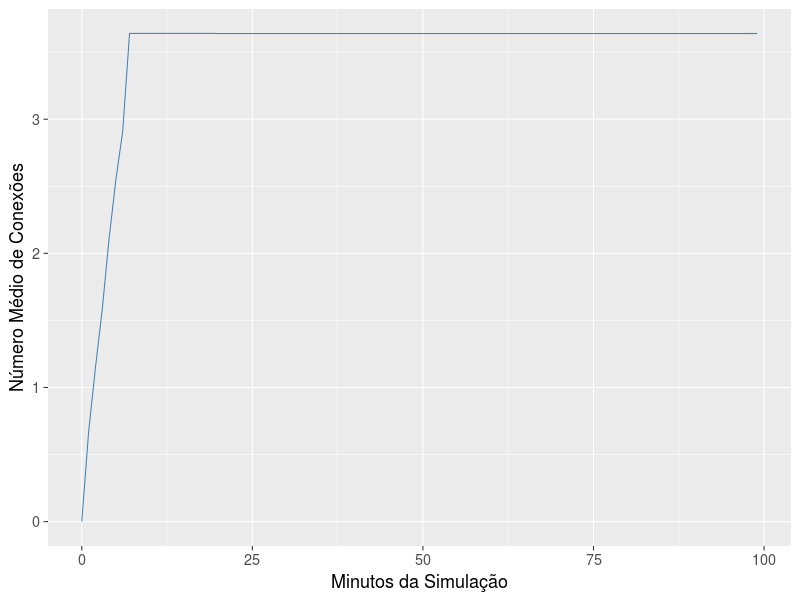
\includegraphics[width=0.6\textwidth]{figuras/chap-uses/num_conexoes.png}
\caption{Mean number of connections during the simulation}
\label{fig:media_conexoes}
\end{figure}

\section{Bus Model Experiments}
\label{sec:mobiity_model}

The InterSCSimulator was used by a study group of a Smart City course to make experiments of a bus mobility model. They created the model based on the real traces of the movement of the buses of S\~ao Paulo provided by the transportation secretariat of the city (SpTrans). The original bus mobility model from InterSCSimulator used the planned intervals to create the buses on the simulation and compared the speed of the buses with the general traffic in the simulation.

However, using the real data from the city, collected by the Automatic Vehicle Location (AVL), the group showed that there are great differences in the planned and real intervals of the city buses. With this data, the group extended the bus mobility model with more accurate data, improving the results of the simulator. Moreover, the students compared the simulated and the real travels times and showed that the results were very close to the real system. Figure \ref{fig:simulation_real_comparison} compares the simulated and the real times.

\begin{figure}[!htb]
\centering
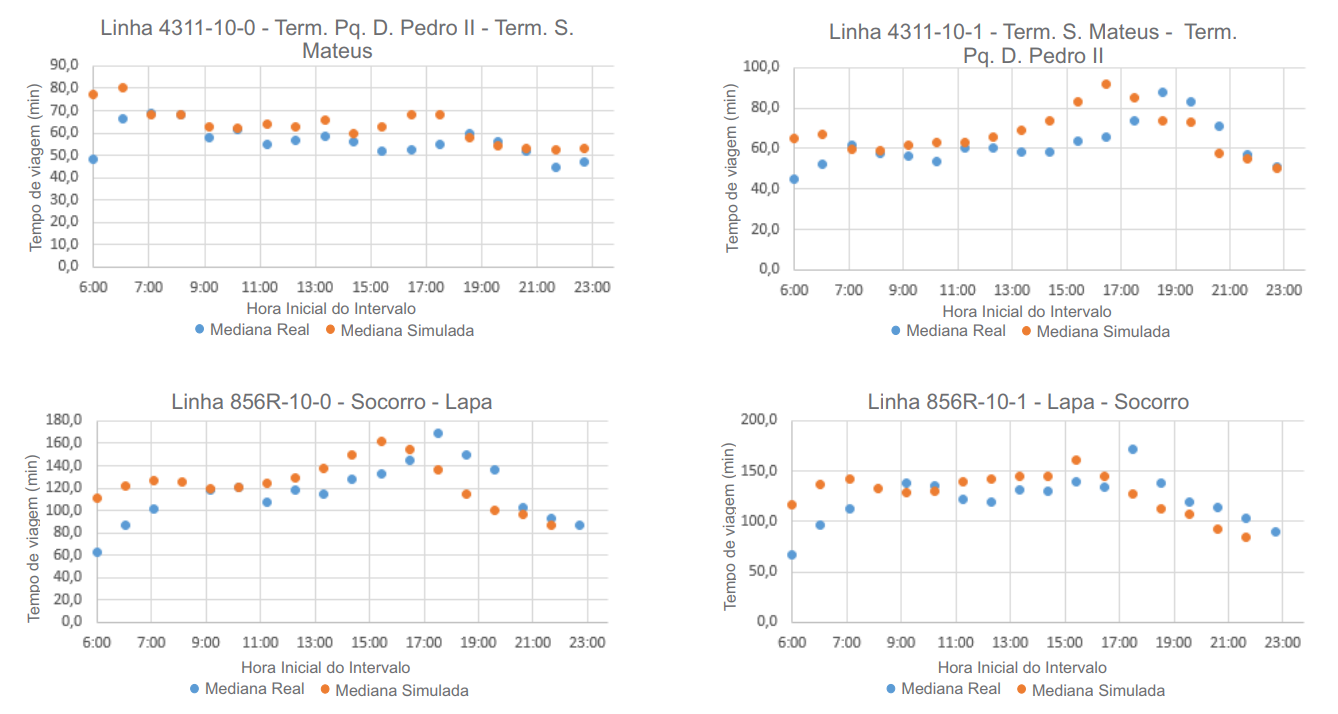
\includegraphics[width=1\textwidth]{figuras/chap-uses/bus_model.png}
\caption{Simulation and Real Time Comparison}
\label{fig:simulation_real_comparison}
\end{figure}

\section{Digital Rails}
\label{sec:digital_rails}

Autonomous vehicles (AVs) technology brings new solutions and challenges for urban mobility. The development and adoption of AVs has the potential to reduce traffic jams and increase traffic safety. However, despite the advancement of automation technology in both research and commercial environments, full autonomous vehicles requiring no human intervention are not expected to be available in the short-term. 

A work investigated the Digital Rails (DR), a proposal to allow AVs to share the roads with regular vehicles, with minimal changes to the current cities infra-structure. DR consists on dedicated lanes for AVs that allows AV platoons to traverse arterial roads at high speeds and synchronized traffic signals coordinates the traffic with regular vehicles. On roads with DR lanes, traffic signals on successive intersections should be synchronized to allow the platoons to travel without stops.The proposal for Digital Rails was first elaborated by designers at a design consultancy firm called Questtonó\footnote{\url{https://www.questtono.com/en/}}. 

The analyses evaluated the impact that such system could have in traffic using simulations based on the city of São Paulo. The DR simulations expanded the InterSCSimulator implementing a couple of features on the simulator such as the synchronized traffic signals, the exclusive AV lanes, and the AV movement model. Figure \ref{fig:dr_network} presents the DR network simulated in the city of S\~ao Paulo.

\begin{figure}[!htb]
\centering
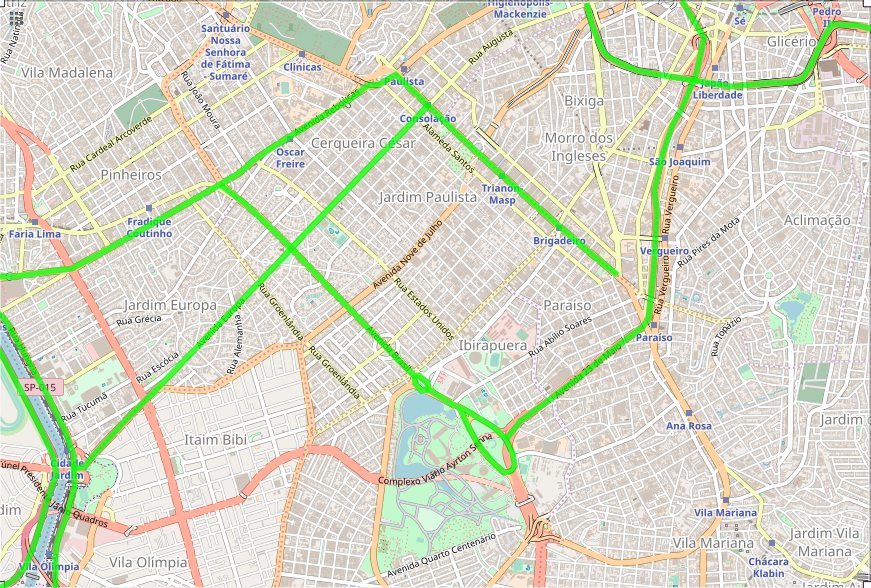
\includegraphics[width=1\textwidth]{figuras/chap-uses/proposal.png}
\caption{DR network simulated in the city of São Paulo}
\label{fig:dr_network}
\end{figure}

To simulate the impact of the DR in the city, it was created a scenario based on the simulation presented in Chapter \ref{cap:sao_paulo}. Four simulations were executed, the first with 0\% of DR vehicles, the second with 25\% and the last with 75\%. As expected, the average travel time increased when the ratio is 0, because the assignment of a lane for DR decreased the road capacity on the selected arterial ways. 
With 25\% of vehicles able to use DR, the average travel time were lower or very similar to the benchmark scenario. For ratios greater than 50\% of vehicles able to use DR, all average times were lower than the benchmark. With 100\% of vehicles able to use DR, the travel times were about 65\% of the benchmark.

We also analyze travel times considering only vehicles that are not able to use DR. Figure \ref{fig:dr-sp-out} shows the evolution of travel times for them. With a ratio of 25\% of vehicles able to use DR, the average travel time is equal or lower than in the benchmark scenario. For ratios higher than 50\%, the average travel time is smaller than in the benchmark scenario. Finally, for 75\% of vehicles able to use DR, the average travel time is between 67\% and 79\% of the benchmark scenario.